\documentclass[11pt,a4paper]{article}
\usepackage{fontspec}
\setmainfont{Source Serif 4}[Path=/home/claude/ref/fonts/, UprightFont=SourceSerif4-Regular.ttf, BoldFont=SourceSerif4-Semibold.ttf, ItalicFont=SourceSerif4-It.ttf]
\setmonofont{IBM Plex Mono}[Path=/home/claude/ref/fonts/, UprightFont=IBMPlexMono-Regular.ttf, BoldFont=IBMPlexMono-Medium.ttf, Scale=0.88]
\usepackage[a4paper,margin=2.4cm]{geometry}
\usepackage{amsmath}
\usepackage{graphicx,booktabs,float,caption,array,xcolor,longtable}
\usepackage{xurl}
\usepackage[hidelinks]{hyperref}
\usepackage[round]{natbib}
\usepackage{setspace}
\setstretch{1.08}
\renewcommand{\topfraction}{0.9}
\renewcommand{\bottomfraction}{0.8}
\renewcommand{\textfraction}{0.1}
\renewcommand{\floatpagefraction}{0.75}
\setlength{\parindent}{0pt}
\setlength{\parskip}{0.55em}
\captionsetup{font=small,labelfont=bf}
\setlength{\bibsep}{3pt}
\urlstyle{same}
\hypersetup{pdftitle={Does Anyone Play Your Town?},pdfauthor={Dr Tristan Hotham}}

\begin{document}
\begin{center}
{\Large\bfseries Does Anyone Play Your Town? The Geography of the Documented Concert Record in the United Kingdom, 1960 to 2025\par}
\vspace{1.2em}
{\large Dr Tristan Hotham\par}
\vspace{0.3em}
{\small Independent researcher\\
ORCID: 0000-0003-4931-9349\\
DOI: https://doi.org/10.5281/zenodo.24113541\par}
\vspace{0.8em}
2026
\end{center}

\begin{quote}
\small
\begin{center}\textbf{Abstract}\end{center}
Open, crowd-sourced archives are attractive sources for the geography of live music, but little is known about where they look. I place every United Kingdom event in the MusicBrainz database, an open music encyclopaedia edited by volunteers, into its local authority and ask which places this record remembers. The record is thin: 7,615 documented concerts from 1960 to 2025, a median of 120 a year since 1980, a small fraction of the concerts that take place. Following a plan written before any area-level count was made, I model documented concerts across all 361 local authorities with Poisson pseudo-maximum likelihood. Documented concerts rise more than in proportion to population (elasticity 1.64, 95\% CI 1.21 to 2.08). Areas with an indoor arena of 10,000 or more seats have 3.8 times the documented concerts of similar areas without one (95\% CI 1.1 to 13.7), a premium larger than in all but 0.4\% of 500 placebo assignments, and the premium is concentrated in tour dates: the 14 arena areas hold 10\% of the population and 53\% of documented tour dates. The expected shadow of arenas on nearby towns is not found in the planned model; it appears only when London is excluded. 70 of the 167 authorities with 150,000 or more residents have no documented tour date. Crowd-sourced concert data describe the geography of attention to live music as much as live music itself, and need coverage audits like this one.

\textbf{Keywords:} live music; concert touring; MusicBrainz; crowd-sourced data; volunteered geographic information; urban scaling; arenas; United Kingdom
\end{quote}

\section{Introduction}\label{sec:intro}
Every live music event leaves a few traces: a poster, a ticket, a review, a setlist, a memory. Some of those traces are now collected in open databases that anyone can edit and anyone can download. MusicBrainz, the open music encyclopaedia maintained by the MetaBrainz Foundation, also records events: concerts, festivals and other performances, each with a date, a venue and the artists who played \citep{metabrainz2026}. For researchers the appeal is obvious. A free, structured, global record of concerts would allow the geography of live music to be mapped at a scale that surveys and venue censuses cannot reach.

This paper asks what such a record actually shows. It takes the United Kingdom, a country with a long and well-documented live music history \citep{frith2013,frith2021} and a mature open-data infrastructure, and asks a question that sounds like a question about music but is really a question about documentation: which towns does the crowd-sourced record of concerts remember, and which does it skip? The title's question, ``does anyone play your town?'', can only be answered here in the form ``has anyone written down that someone played your town?''. The distinction is the paper's subject.

I place each of the 11,329 MusicBrainz events located in the United Kingdom in one of the 361 local authorities and count the 7,615 concerts dated 1960 to 2025. Before computing any area-level count I wrote an analysis plan with four expectations: that documented concerts rise more than in proportion to population, as many urban quantities do \citep{bettencourt2007}; that areas with a large arena have more and that areas close to such an arena have fewer (a shadow, in the language of central place theory; \citealp{christaller1966}); that tour dates are more concentrated in large places than other documented concerts; and that concentration has grown over time.

Three findings stand out. First, the documented record follows size steeply: doubling an area's population goes with about 213\% more documented concerts. Second, the record is organised around the arena circuit: the 14 local authorities with an indoor arena of 10,000 or more seats hold 10\% of the population but 38\% of documented concerts and 53\% of documented tour dates, and the premium keeps its sign in every robustness check, although its interval includes one in the checks that remove the heaviest documenters. Third, the shadow I expected is not there in the planned model; it emerges only when London, where a dense cluster of famous venues sits close to two arenas, is set aside. I report that as exploratory.

The contribution is twofold. Substantively, the paper offers the first area-level description, to my knowledge, of the UK's documented concert record across six decades, and shows how strongly it is shaped by the arena circuit and by a handful of fan-built venue archives. Methodologically, it offers a coverage audit for a crowd-sourced cultural dataset, in the tradition of work on the uneven geography of volunteered information \citep{goodchild2007,haklay2010,graham2014}, and argues that any use of such data for the geography of live music must begin with one.

Section~\ref{sec:lit} reviews work on the geography of live music, urban scaling and volunteered information. Section~\ref{sec:data} describes the data and the coverage audit, Section~\ref{sec:design} the pre-specified design, Section~\ref{sec:results} the results and Section~\ref{sec:robust} the robustness and placebo checks. Section~\ref{sec:disc} discusses what the documented record can and cannot say.

\section{Background and literature}\label{sec:lit}
\subsection{The geography of live music}
Geographers came late to music. \citet{hudson2006} described how, for many years, human geography paid little attention to music, and how a wave of work since the 1990s has studied music's ties to place, identity and economy. \citet{connell2003} gave the field its first comprehensive account, from local scenes to world music, and \citet{cohen2007} showed for Liverpool how popular music is bound up with a city's decline and renewal. Economic geographers have mapped where the music industries cluster. \citet{florida2010} found that musicians and music businesses in the United States concentrated in a small number of large regional centres between 1970 and 2000, with support for both scale and scope effects, and \citet{watson2008} showed how London's recorded music industry depends on face-to-face proximity.

Live music has its own economy and its own geography. In the United Kingdom, a research programme on the history of live music has traced the industry from the dance halls of the 1950s to the arena tours and corporate promoters of the 2000s \citep{frith2013,frith2021}. \citet{brennan2011} described the promoter as the pivot of that economy and warned that corporate consolidation could weaken the ecology of small and large venues on which live music depends. \citet{behr2016} developed that ecological view through three Scottish concerts in venues of different size, from King Tut's in Glasgow to the 12,000-seat Hydro. The UK Live Music Census of 2017 combined a 24-hour snapshot of live music in three cities with national surveys, and found at least 241 spaces where live music is played in Glasgow alone \citep{webster2018}. Festivals have become a large part of the live calendar \citep{anderton2018}.

Economists have documented the shift of income from recordings to concerts. \citet{krueger2005} showed concert prices rising much faster than general prices from the late 1990s and tied the change to the erosion of the complementarity between records and concerts, and \citet{connolly2006} described the concentration of concert revenue among the top performers. \citet{mortimer2012} found that file sharing reduced album sales while raising concert demand, especially for small artists, and \citet{holt2010} examined the economy of live music in the digital age. One consequence is the arena tour as the central form of the business for the biggest acts, played in a small set of large venues.

\subsection{Size, scaling and central places}
The expectation that larger places host disproportionately more concerts has two sources. Urban scaling research finds that many socio-economic quantities, from wages to patents, scale superlinearly with city population, with exponents typically between about 1.1 and 1.3 \citep{bettencourt2007,bettencourt2013}. Live music, which depends on audiences, networks of musicians and specialised venues, is a plausible member of that class. Central place theory adds a hierarchy: higher-order functions with large thresholds are found only in a few large centres, which serve the towns around them \citep{christaller1966}. An arena of 10,000 seats is such a function. If audiences travel to the arena city, towns near it should host fewer large concerts than towns of the same size far from one: a shadow.

\subsection{Volunteered information and its uneven coverage}
MusicBrainz began as an open, community-maintained database of music metadata \citep{swartz2002}. Like OpenStreetMap and Wikipedia, it belongs to the family of volunteered information that \citet{goodchild2007} called ``citizens as sensors''. Such data can be accurate where they exist \citep{haklay2010}, but their coverage is uneven: \citet{graham2014} found that geotagged Wikipedia content is highly unequal across the world, and that some places fall far below what their connectivity and wealth would predict. Coverage follows the interests and the reach of the people who contribute. For concert data this means that a record will be fullest for the acts that fans care most about and for venues whose histories someone has chosen to type in. No study I know of has audited the geography of MusicBrainz's event data.

\subsection{Expectations}
The analysis plan (Section~\ref{sec:design}) states four hypotheses: H1, documented concerts scale superlinearly with population; H2, arena areas have more documented concerts and other areas closer to an arena have fewer; H3, tour dates are more concentrated in large places than other documented concerts; H4 (exploratory), concentration has grown over time.

\section{Data}\label{sec:data}
\subsection{MusicBrainz events and places}
The MusicBrainz JSON data dumps of 2026 contain one record per line for each entity \citep{metabrainz2026}. I streamed the event and place dumps directly from their compressed archives without unpacking them. The event dump holds 129,282 events worldwide, of which 85,436 are typed Concert and 32,137 Festival; 114,144 are linked to a place by a ``held at'' relationship and 89,475 to a place with coordinates. Each event carries a date (the start of its life span), a cancelled flag, and relationships to artists (main performer, support act and others), places and areas. The place dump holds 84,565 places with their type, coordinates and area.

\subsection{What a documented concert is}
A MusicBrainz event is a record created by a volunteer editor, with a name, a type, a date and relationships to artists and a place; like the rest of the database it is openly edited \citep{swartz2002,metabrainz2026}. Editors may enter an event because they attended it, because it produced a recording, or because they are working through a source such as a tour list or a venue history; the dump does not say which. Two consequences follow. First, an event exists in the record only if someone cared enough about that act, that venue or that night to enter it; the record is a sample selected on the interests of its editors. Second, editors tend to work in batches: a full tour of a favourite act, the complete listing of a venue they loved, the concerts that produced a live album. Batches create the spikes visible in Figure~\ref{fig:coverage} and the heavy weight of a few acts and venues described below. Neither feature is a flaw for MusicBrainz's purposes, which are to describe music and its context accurately, but both matter when its events are counted.

\subsection{Placing events in the United Kingdom}
An event is in the United Kingdom if its venue's coordinates fall inside one of the 361 local authority districts of December 2023 (ONS and OSNI boundaries; points within 2 km of the coast go to the nearest authority). Where a venue has no coordinates, or an event has only a ``held in'' area, I place it at the largest UK settlement in Wikidata whose name matches the area's name, provided the area carries a GB ISO 3166-2 code. 11,329 events are placed: 10,425 by venue coordinates and 904 (8\%) by area name; 350 events in a broad UK box fell outside every authority (mostly in Ireland and the Isle of Man) and 147 with a GB area could not be placed.

The outcome is the documented concert: an event typed Concert, not cancelled, with a start date from 1960 to 2025. There are 7,615 such concerts. 2026 is excluded because the dump contains announced future dates. Festivals and untyped events enter a robustness check.

\subsection{Coverage audit}
Figure~\ref{fig:coverage} shows documented UK concerts by year. The record grows from a few concerts a year in the 1960s to a median of 120 a year between 1980 and 2023 (minimum 28), with spikes in years for which whole tours were entered date by date: 582 in 1998, the maximum, and 485 in 2024. Even the spikes are a small fraction of the UK's live music. The 2017 census found at least 241 spaces for live music in Glasgow, 137 in Newcastle and Gateshead and 110 in Oxford \citep{webster2018}; across 66 years MusicBrainz documents concerts at 57, 22 and 6 venues in those places.

The record is also concentrated. The ten most documented main performers (led by Barry Manilow with 234 UK concerts, Girls Aloud with 144 and Take That with 119) account for 12\% of documented concerts, and the ten most documented venues for 26\%. The second of those venues is the West Runton Pavilion in North Norfolk, with 335 concerts, all dated 1975 to 1983: a single venue archive that makes a rural district of 102,979 people the fourth most documented authority in the UK. Television studios also appear as venues for recorded performances. I keep all of these, because they are what the record is, and test their influence in Section~\ref{sec:robust}.

\begin{figure}[tbp]\centering
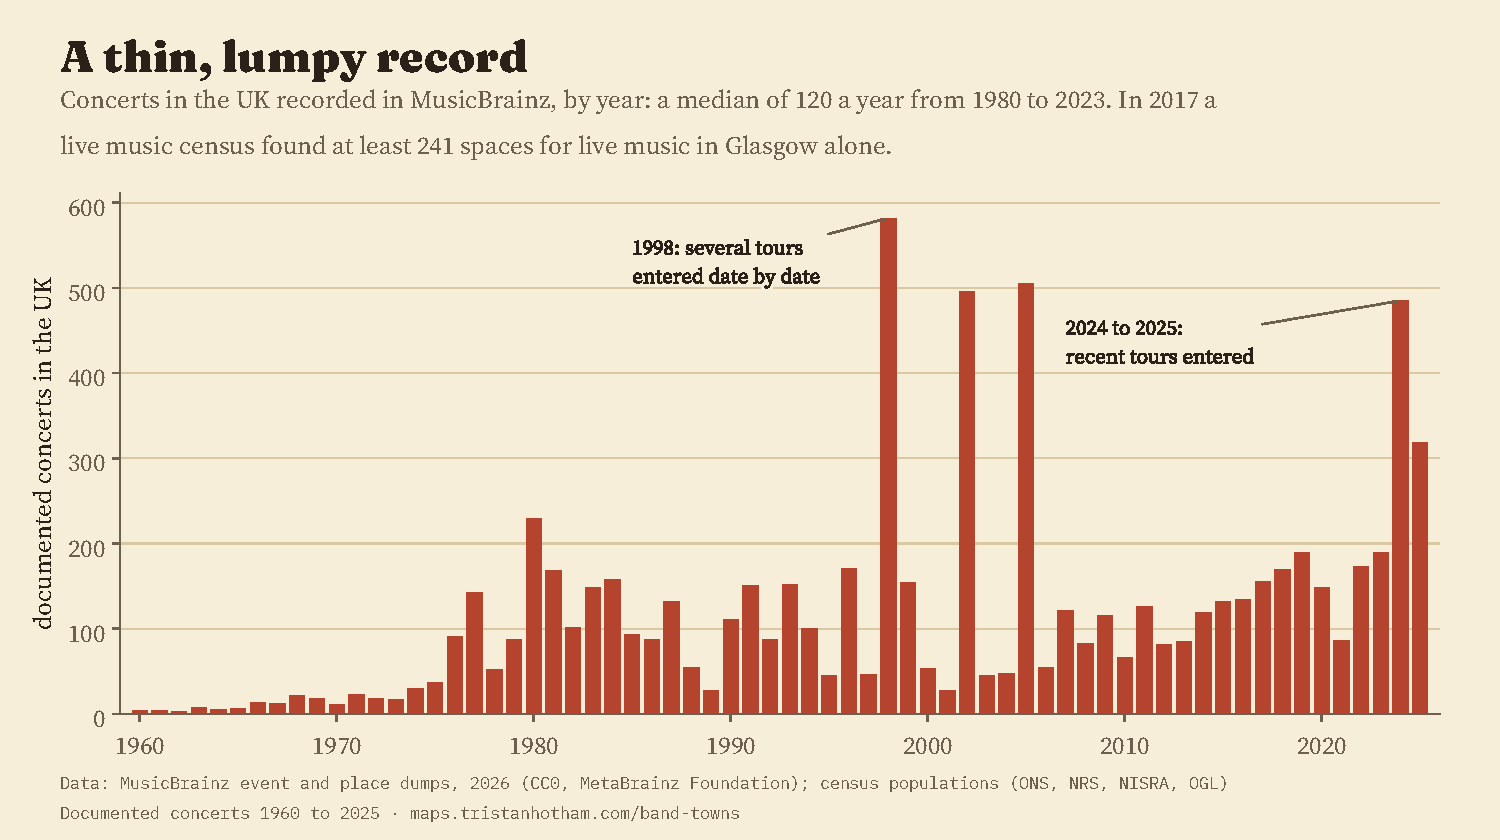
\includegraphics[width=0.92\textwidth]{f_coverage.pdf}
\caption{Documented UK concerts in MusicBrainz by year, 1960 to 2025.}\label{fig:coverage}
\end{figure}

\subsection{Population, arenas and distance}
Population is the census count of usual residents by local authority (2021 in England, Wales and Northern Ireland; 2022 in Scotland; ONS, NISRA and NRS). Arenas come from an outside source, not from MusicBrainz: the UK indoor arenas with a capacity of 10,000 or more in Wikipedia's list of indoor arenas in the United Kingdom, retrieved in 2026 \citep{wikiarenas2026}. There are 15, in 14 local authorities (Table~\ref{tab:arenas}). Distance to an arena is the great-circle distance in kilometres from each authority's representative point to the nearest arena, floored at 1 km.

\begin{table}[tbp]\centering\small\caption{UK indoor arenas of 10,000 or more seats (Wikipedia list, retrieved 2026) and the local authority containing each.}\label{tab:arenas}\begin{tabular}{llrr}\toprule Arena & Local authority & Capacity & Opened\\\midrule
bp pulse LIVE (NEC) & Solihull & 15,685 & 1980\\
Utilita Arena Birmingham & Birmingham & 15,800 & 1991\\
Coventry Building Society Arena & Coventry & 10,000 & 2005\\
first direct arena & Leeds & 13,781 & 2013\\
M\&S Bank Arena & Liverpool & 11,000 & 2008\\
The O2 Arena & Greenwich & 20,000 & 2007\\
OVO Arena Wembley & Brent & 12,500 & 1934\\
AO Arena & Manchester & 23,000 & 1995\\
Co-op Live & Manchester & 23,500 & 2024\\
Utilita Arena Newcastle & Newcastle upon Tyne & 11,400 & 1995\\
Motorpoint Arena Nottingham & Nottingham & 10,000 & 2000\\
Utilita Arena Sheffield & Sheffield & 13,600 & 1991\\
SSE Arena & Belfast & 10,800 & 1999\\
P\&J Live & Aberdeen City & 15,000 & 2019\\
OVO Hydro & Glasgow City & 14,300 & 2013\\
\bottomrule\end{tabular}\end{table}

\section{Research design}\label{sec:design}
\subsection{Analysis plan}
The plan was written in the study's notes after the coverage audit and before any area-level count was computed. It fixed the unit, the outcome, the exposures, the models, the robustness checks and what would count against each hypothesis. Anything not in the plan is labelled exploratory.

\subsection{Unit and outcome}
The unit is the local authority district (N = 361), chosen because it partitions the UK and has a clean population denominator. The outcome is the count of documented concerts, 1960 to 2025. Of the 361 authorities, 200 have at least one documented concert and 161 have none.

\subsection{Models}
All models are Poisson pseudo-maximum likelihood (PPML) regressions, which estimate log-linear models for counts consistently under heteroskedasticity and handle zeros without transformation \citep{santos2006}. With one observation per authority, standard errors are heteroskedasticity-robust (HC1).

\textbf{H1 (size).} M1: concerts $\sim \log(\text{population})$ + nation fixed effects. The coefficient on log population is the elasticity; H1 predicts it exceeds 1, and the test is against 1.

\textbf{H2 (arenas and shadow).} M2, the main specification: concerts $\sim \log(\text{population})$ + arena + $\log(\text{distance to nearest arena})$ + nation fixed effects. H2 predicts a positive arena coefficient and a positive distance coefficient (more concerts farther from an arena, all else equal). The fitted values of M2 define each authority's expected count, used for the map.

\textbf{H3 (touring).} A tour is an artist-year with five or more documented UK concerts as main performer; tour dates are the concerts on such tours. There are 438 tours by 326 artists (median 8 dates in 6 authorities). M3 stacks two outcomes per authority, tour dates and other concerts, with outcome-specific intercepts and interactions of log population, arena and log distance with a tour indicator, and standard errors clustered by authority. H3 predicts a positive log population $\times$ tour interaction.

\textbf{H4 (time, exploratory).} M1 and M2 by decade, with the arenas open in each decade.

\subsection{Threats to inference}
The design is cross-sectional and descriptive. Population is measured in 2021 or 2022 for every decade. The outcome is the record, and the record's coverage is the main threat: a single prolific volunteer can make a town. The robustness checks are chosen to probe that threat (capping each artist per area, dropping the most documented acts, counting venues and acts instead of concerts), and a placebo assigns arena status to random authorities of similar size. Nothing here identifies a causal effect of an arena; the estimates describe where documented concerts are.

\section{Results}\label{sec:results}
\subsection{Size}
Documented concerts rise steeply with population (Figure~\ref{fig:scaling}; Table~\ref{tab:main}). In M1 the elasticity is 1.64 (95\% CI 1.21 to 2.08; N = 361), significantly above 1 ($p$ = 0.004): an authority with twice the population has about 213\% more documented concerts. H1 is supported. The elasticity is higher than the 1.1 to 1.3 typical of socio-economic quantities in urban scaling studies \citep{bettencourt2007}, which is what one would expect if documentation itself favours big places on top of the concerts. The 161 authorities with no documented concert are home to 21.8 million people, 33\% of the population.

\begin{figure}[tbp]\centering
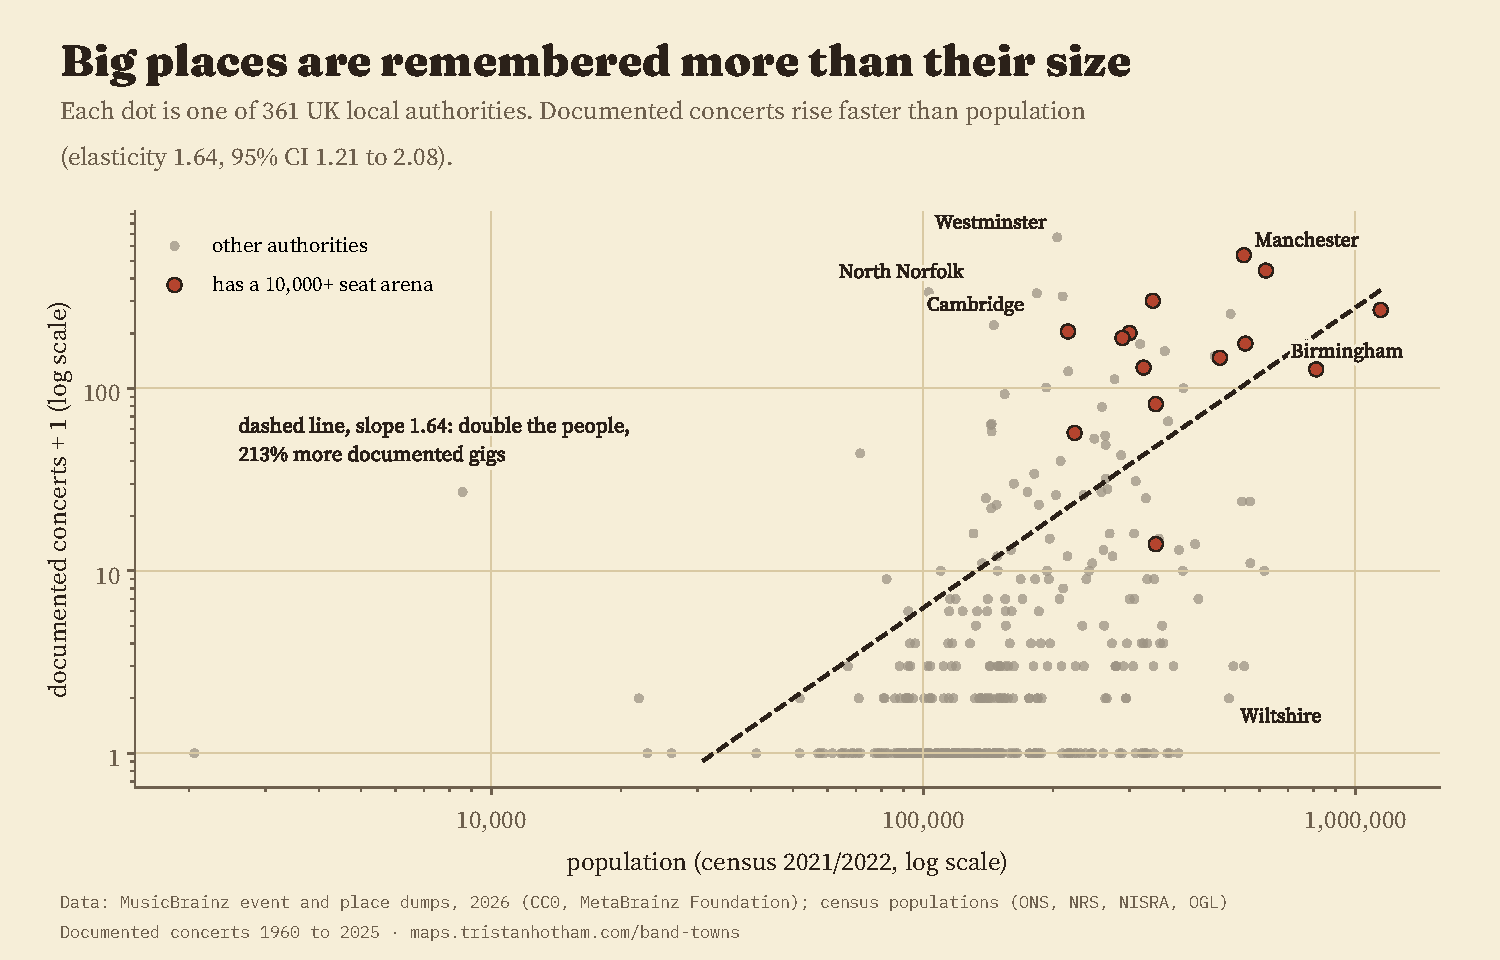
\includegraphics[width=0.92\textwidth]{f_scaling.pdf}
\caption{Documented concerts (plus one) against population, by local authority, log scales. Red: authorities with an indoor arena of 10,000+ seats. Dashed line: slope 1.64.}\label{fig:scaling}
\end{figure}

\begin{table}[tbp]\centering\small\caption{Main models (PPML; nation fixed effects; HC1 standard errors for M1 and M2, clustered by authority for M3). Coefficients with 95\% CI; for arena and distance terms the rate ratio is also shown.}\label{tab:main}\begin{tabular}{p{6.3cm}lrr}\toprule Term & Estimate [95\% CI] & $p$ & N\\\midrule
M1: log population (elasticity) & 1.64 [1.21, 2.08] & $<$0.001 & 361\\
\quad test of elasticity = 1 & z = 2.90 & 0.004 & \\\midrule
M2: log population & 0.92 [0.48, 1.36] & $<$0.001 & 361\\
M2: arena in the authority (rate ratio) & 3.80 [1.05, 13.73] & 0.041 & 361\\
M2: log distance to nearest arena & -0.22 [-0.68, 0.24] & 0.345 & 361\\
M2: pseudo-$R^2$ (deviance) & 0.38 & & \\\midrule
M3: log population (other concerts) & 0.74 [0.22, 1.27] & 0.006 & 722\\
M3: log population $\times$ tour & 0.31 [-0.22, 0.84] & 0.257 & 722\\
M3: arena (other concerts, rate ratio) & 1.35 [0.27, 6.75] & 0.715 & 722\\
M3: arena $\times$ tour (ratio of rate ratios) & 7.02 [2.26, 21.76] & $<$0.001 & 722\\
M3: log distance (other concerts) & -0.39 [-1.00, 0.23] & 0.220 & 722\\
M3: log distance $\times$ tour & 0.35 [-0.14, 0.85] & 0.160 & 722\\
\bottomrule\end{tabular}\end{table}

\subsection{Arenas and the missing shadow}
In M2, conditional on population and nation, an authority with an arena has 3.80 times the documented concerts of one without (95\% CI 1.05 to 13.73, $p$ = 0.041). The arena authorities hold 9.8\% of the UK's population and 37.6\% of its documented concerts (Figure~\ref{fig:arenas}). The distance coefficient, however, is -0.22 (95\% CI -0.68 to 0.24, $p$ = 0.35): if anything, authorities farther from an arena have fewer documented concerts, not more. The shadow part of H2 is not supported in the planned specification. With the population elasticity conditional on arenas, M2's elasticity falls to 0.92 (95\% CI 0.48 to 1.36): much of the superlinearity in M1 runs through the arena cities.

\begin{figure}[tbp]\centering
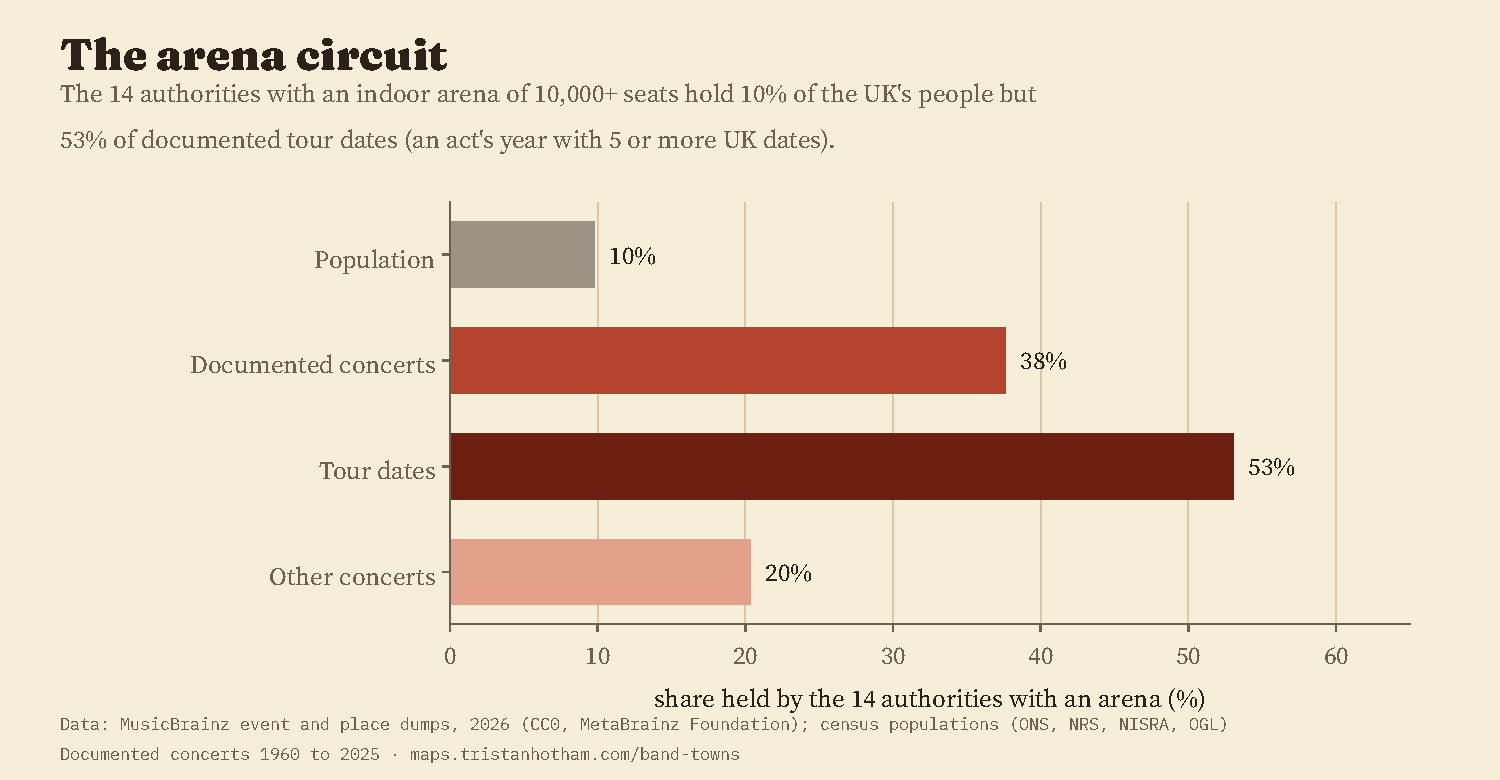
\includegraphics[width=0.85\textwidth]{f_arenas.pdf}
\caption{Shares of the UK's population, documented concerts, tour dates and other concerts held by the 14 authorities with an indoor arena of 10,000+ seats.}\label{fig:arenas}
\end{figure}

Figure~\ref{fig:map} maps documented concerts against M2's expectation. The largest surpluses relative to expectation (among authorities expected to have at least five) are North Norfolk (335 documented against 6.2 expected), Westminster (671 against 21.0), Cambridge (221 against 9.9) and Hammersmith and Fulham (331 against 20.4): one venue archive, the Royal Albert Hall's borough, the Corn Exchange's city and the borough of the Hammersmith Apollo. The largest shortfalls are authorities with no documented concert despite an expectation of dozens: Ealing (43.6 expected), Barnet (40.4) and Sandwell (35.8), outer London boroughs and a West Midlands borough whose residents can reach central venues easily. By a Poisson test at the 1\% level, 42 authorities have more documented concerts than expected and 252 fewer; the second number shows how far the record is from a smooth function of size.

\begin{figure}[tbp]\centering
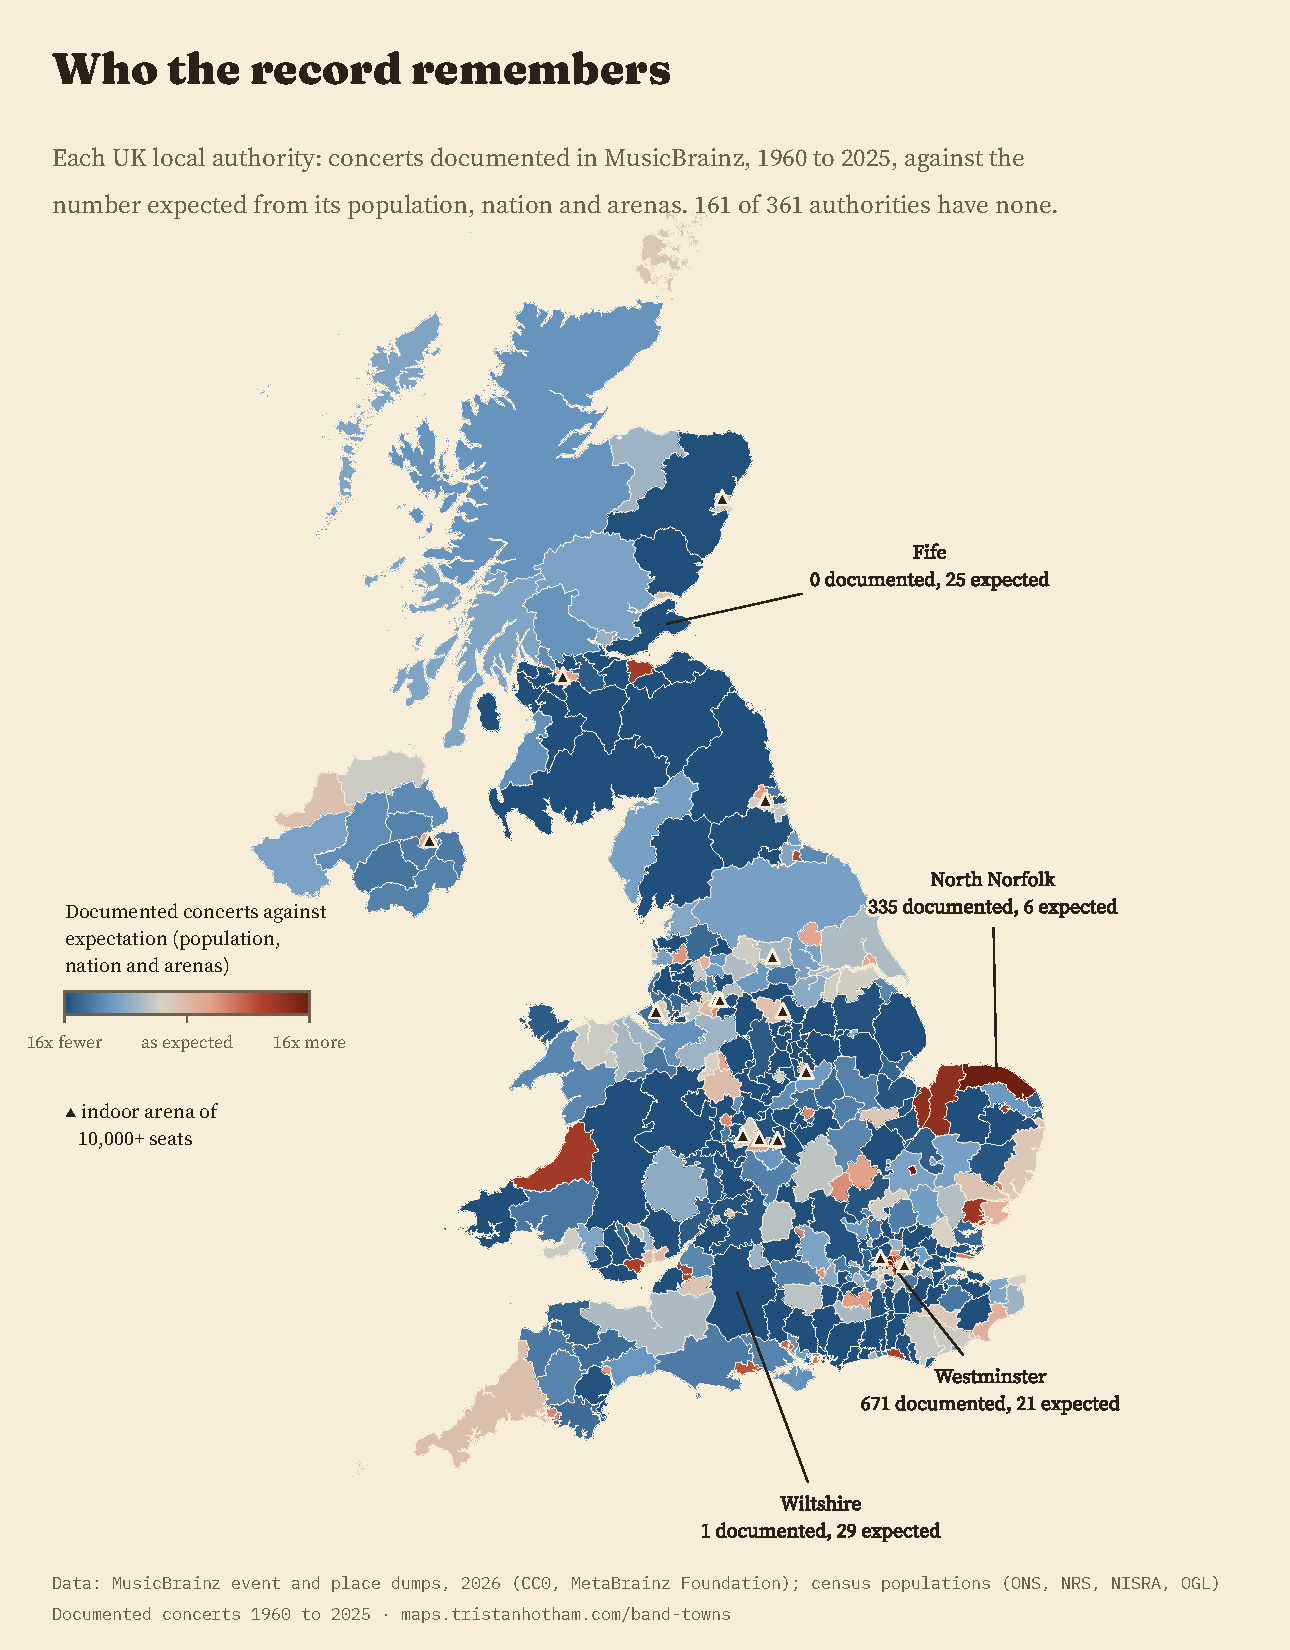
\includegraphics[width=0.75\textwidth]{f_map.pdf}
\caption{Documented concerts against the M2 expectation, by local authority, 1960 to 2025. Triangles: indoor arenas of 10,000+ seats.}\label{fig:map}
\end{figure}

\subsection{Touring}
Tour dates make up 4,022 of the 7,615 documented concerts. In M3 the population elasticity of other concerts is 0.74 and that of tour dates 1.05; the difference, 0.31 (95\% CI -0.22 to 0.84, $p$ = 0.26), is positive but its interval includes zero. H3, as specified, is not supported. What distinguishes tour dates is not population but arenas: the arena premium for tour dates is 7.0 times that for other concerts (95\% CI 2.3 to 21.8). Estimated separately, arena authorities have 8.9 times the tour dates of comparable authorities and 1.5 times the other concerts, an interval for the latter that comfortably includes one. The arena authorities hold 53\% of tour dates and 20\% of other concerts.

Measured by the share of the ten leading authorities, tour dates are in fact less concentrated (49\%) than other concerts (59\%), because other concerts are dominated by a few venue archives (West Runton, the Royal Albert Hall, the Cambridge Corn Exchange). The touring map is a circuit of arena cities plus a ring of mid-sized towns; the non-touring map is a scatter of places with an archivist. 143 authorities have at least one documented tour date; 70 of the 167 with 150,000 or more residents have none (Figure~\ref{fig:skipped}), and the authorities with no documented tour date are home to 48\% of the population.

\begin{figure}[tbp]\centering
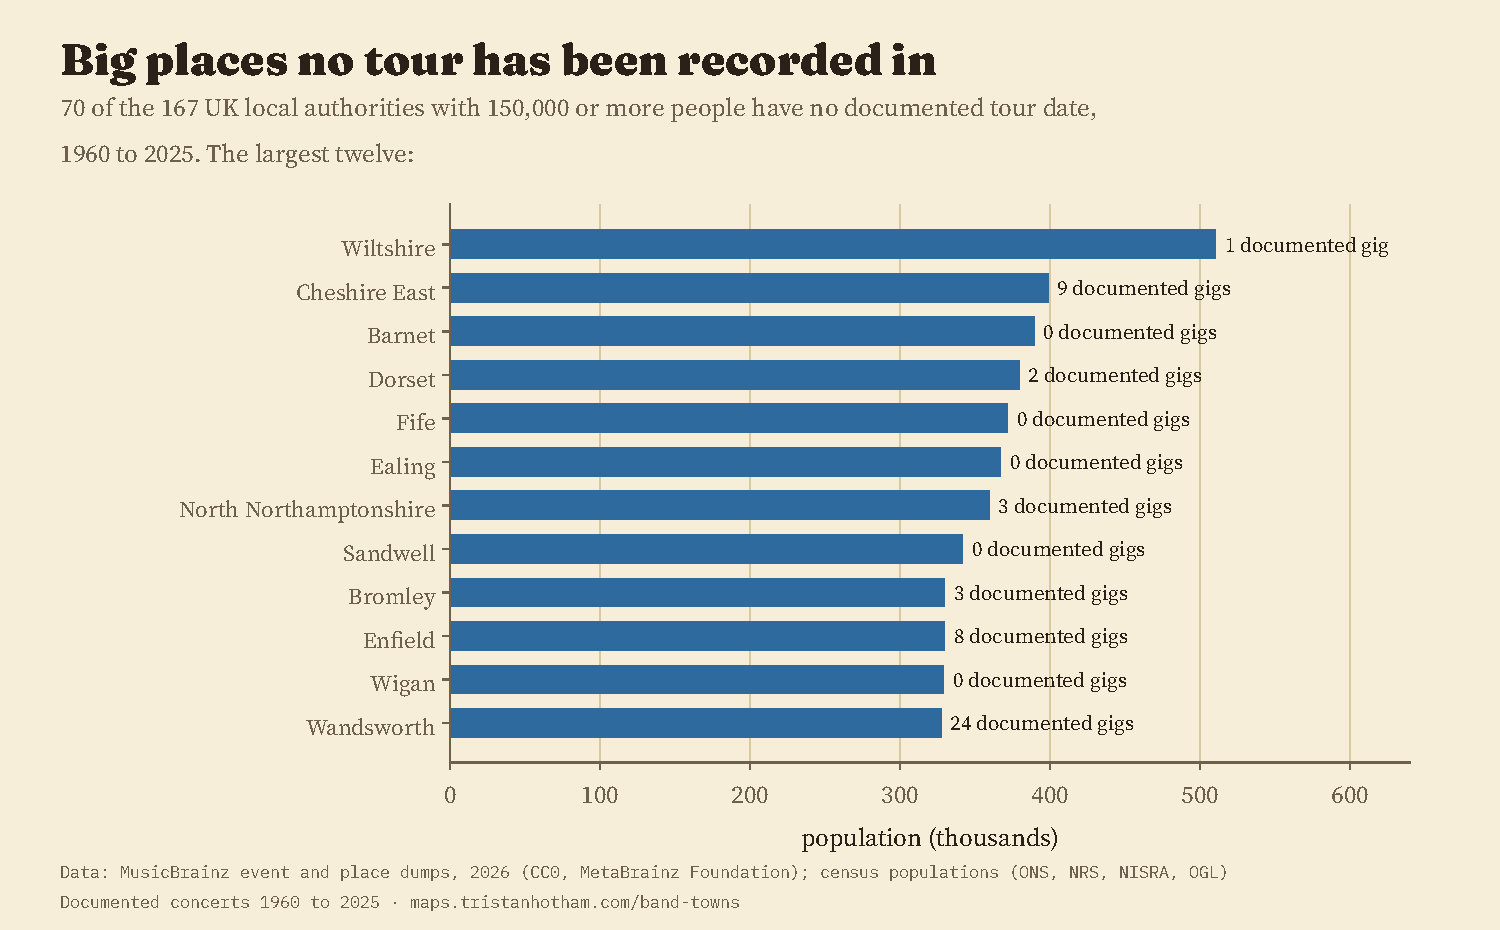
\includegraphics[width=0.85\textwidth]{f_skipped.pdf}
\caption{The twelve most populous authorities with no documented tour date, 1960 to 2025, with their documented concerts of any kind.}\label{fig:skipped}
\end{figure}

\subsection{Over time}
Figure~\ref{fig:decades} and Table~\ref{tab:decades} report the decade models (exploratory). The population elasticity is 0.84 in the 1970s with a very wide interval, then 1.58 in the 1980s, 1.42 in the 1990s and between 1.69 and 1.94 from the 2000s on, every decade from the 2000s with an interval above one. The share of documented concerts in the ten leading authorities falls from 0.84 in the 1970s (when West Runton dominates) to about half from the 1980s. The decade estimates are consistent with growing concentration on large places after the arena era began, but the 1970s interval is too wide to call it a trend, and the composition of the record changes from decade to decade.

\begin{figure}[tbp]\centering
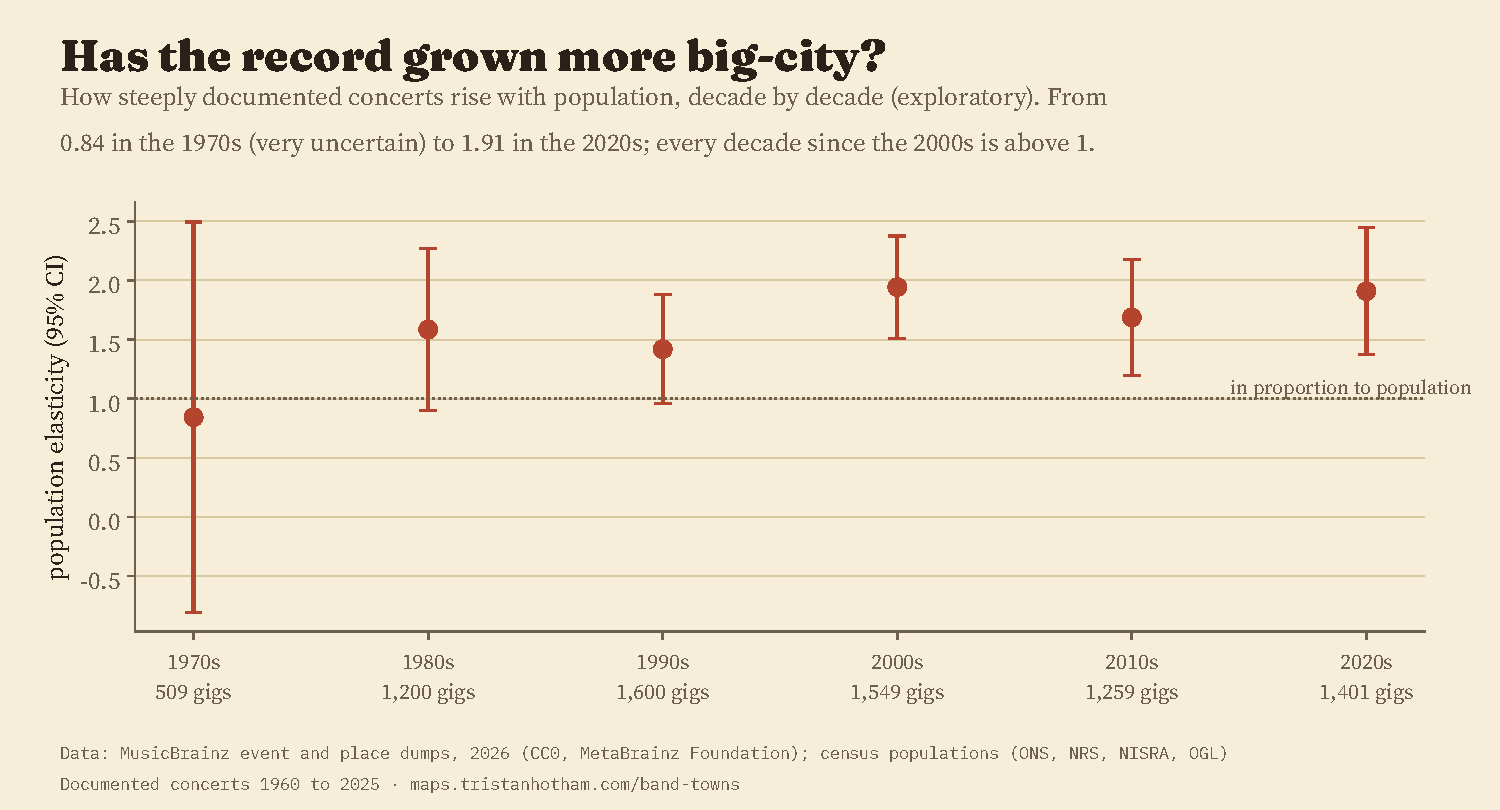
\includegraphics[width=0.85\textwidth]{f_decades.pdf}
\caption{Population elasticity of documented concerts by decade (M1, exploratory), with 95\% intervals.}\label{fig:decades}
\end{figure}

\begin{table}[tbp]\centering\footnotesize\caption{Decade models (exploratory): documented concerts, authorities with any, M1 elasticity, and M2 arena rate ratio and log-distance coefficient using arenas open by the decade; share in the ten leading authorities. N = 361 per decade.}\label{tab:decades}\begin{tabular}{lrrlllr}\toprule Decade & Concerts & Areas & Elasticity & Arena RR & Log distance & Top 10\\\midrule
1970s & 509 & 49 & 0.84 [-0.81, 2.49] & 0.92 [0.03, 26.05] & -0.24 [-1.01, 0.53] & 84\%\\
1980s & 1,200 & 91 & 1.58 [0.90, 2.27] & 8.91 [0.99, 80.50] & -0.06 [-0.61, 0.50] & 55\%\\
1990s & 1,600 & 124 & 1.42 [0.96, 1.88] & 2.94 [0.76, 11.34] & -0.29 [-0.81, 0.22] & 51\%\\
2000s & 1,549 & 107 & 1.94 [1.51, 2.38] & 3.97 [1.29, 12.23] & -0.21 [-0.55, 0.13] & 48\%\\
2010s & 1,259 & 90 & 1.69 [1.20, 2.17] & 2.25 [0.58, 8.72] & -0.56 [-1.03, -0.09] & 60\%\\
2020s & 1,401 & 92 & 1.91 [1.37, 2.45] & 2.22 [0.51, 9.70] & -0.67 [-1.09, -0.24] & 62\%\\
\bottomrule\end{tabular}\end{table}

\section{Robustness}\label{sec:robust}
Table~\ref{tab:robust} and Figure~\ref{fig:robust} report M2 under each pre-specified check. The arena premium is positive in every check; its interval excludes one in the main model, the negative binomial model, the models using only coordinate-placed events, the wider event definition, distinct venues, and each leave-one-nation-out model except dropping England (which leaves 65 authorities); it includes one when each artist is capped at three concerts per authority, when the ten most documented acts are dropped, in 2000 to 2025 alone, and for distinct performers. I therefore describe the premium as large and consistent in sign but sensitive to the heaviest documenters.

The distance coefficient tells a different story. In the main model and most checks it is negative with an interval spanning zero. It turns positive, as H2 predicted, in two checks: without the 33 London boroughs (0.65, 95\% CI 0.27 to 1.02) and with log distance to central London as a control (0.44, 95\% CI 0.01 to 0.86). London combines two arenas with a dense cluster of famous theatres and halls, so its boroughs are close to an arena and heavily documented at once, which masks any shadow elsewhere. In these specifications, towns farther from an arena have more documented concerts than towns of the same size close to one; because neither was the planned specification, I treat this as exploratory.

\begin{figure}[tbp]\centering
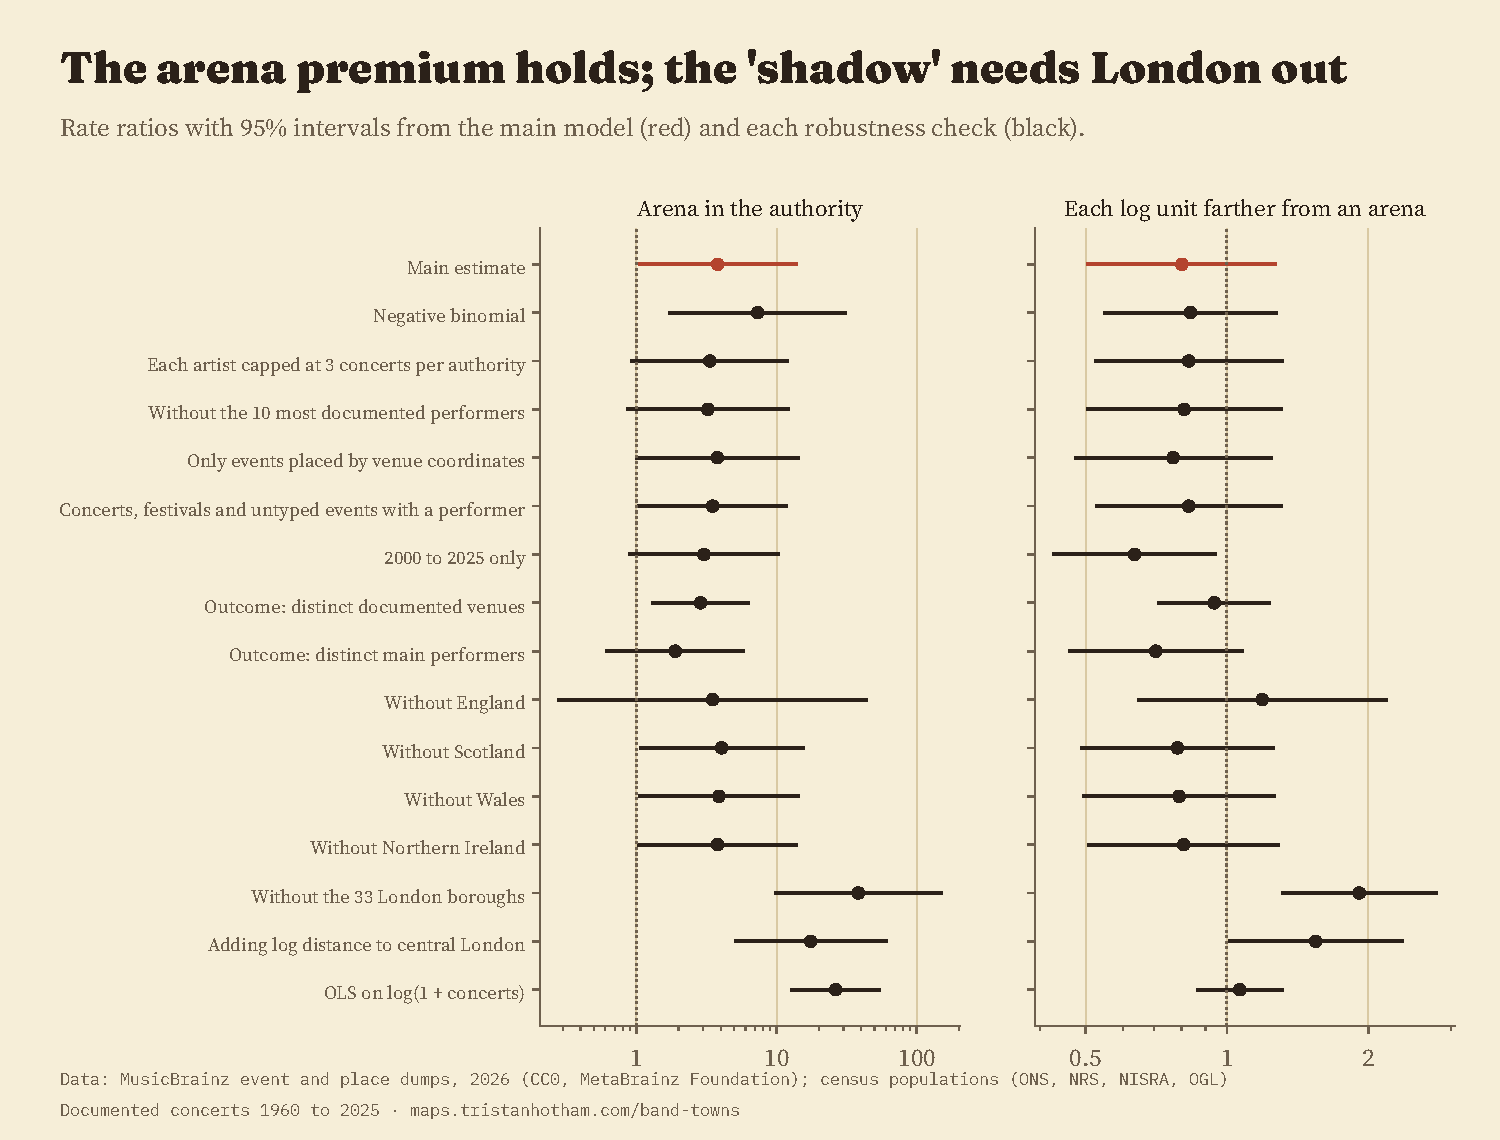
\includegraphics[width=0.95\textwidth]{f_robust.pdf}
\caption{M2 rate ratios for the arena dummy and log distance to the nearest arena under each robustness check, with 95\% intervals.}\label{fig:robust}
\end{figure}

\begin{table}[tbp]\centering\footnotesize\caption{Robustness of M2: arena rate ratio and log-distance coefficient with 95\% CI. The OLS row reports exponentiated OLS coefficients on log(1 + concerts).}\label{tab:robust}\begin{tabular}{p{6.2cm}llr}\toprule Check & Arena rate ratio & Log distance & N\\\midrule
Main estimate (M2) & 3.80 [1.05, 13.73] & -0.22 [-0.68, 0.24] & 361\\\midrule
Negative binomial & 7.33 [1.74, 30.86] & -0.18 [-0.60, 0.24] & 361\\
Each artist capped at 3 concerts per authority & 3.34 [0.94, 11.94] & -0.19 [-0.64, 0.27] & 361\\
Without the 10 most documented performers & 3.24 [0.88, 12.00] & -0.21 [-0.68, 0.26] & 361\\
Only events placed by venue coordinates & 3.79 [1.01, 14.20] & -0.26 [-0.74, 0.21] & 361\\
Concerts, festivals and untyped events with a performer & 3.50 [1.04, 11.78] & -0.19 [-0.64, 0.26] & 361\\
2000 to 2025 only & 3.04 [0.89, 10.31] & -0.45 [-0.85, -0.06] & 361\\
Outcome: distinct documented venues & 2.87 [1.31, 6.28] & -0.06 [-0.33, 0.21] & 361\\
Outcome: distinct main performers & 1.89 [0.62, 5.77] & -0.35 [-0.77, 0.07] & 361\\
Without England & 3.50 [0.28, 43.67] & 0.17 [-0.43, 0.78] & 65\\
Without Scotland & 4.06 [1.07, 15.39] & -0.24 [-0.71, 0.23] & 329\\
Without Wales & 3.88 [1.07, 14.13] & -0.23 [-0.70, 0.23] & 339\\
Without Northern Ireland & 3.80 [1.05, 13.76] & -0.21 [-0.68, 0.25] & 350\\
Without the 33 London boroughs & 38.35 [9.89, 148.70] & 0.65 [0.27, 1.02] & 328\\
Adding log distance to central London & 17.52 [5.10, 60.16] & 0.44 [0.01, 0.86] & 361\\
OLS on log(1 + concerts) & 26.43 [12.95, 53.95] & 0.06 [-0.14, 0.27] & 361\\
\bottomrule\end{tabular}\end{table}

\textbf{Placebo arenas.} In 500 draws, I gave arena status to one random non-arena authority in the same population decile as each real arena authority and recomputed distances to these placebo centres. The real arena coefficient exceeds the placebo coefficient in all but 0.4\% of draws, so the premium is not simply a feature of any set of large places. The real distance coefficient is higher than 94\% of placebo distance coefficients (placebo mean -0.46): the negative distance gradient in M2 is what one finds around any set of large places, not something specific to arenas.

\textbf{Recording studios.} As an exploratory falsification I fitted M2 to the 569 UK places typed Studio in MusicBrainz. Studios fall off more steeply with distance from an arena than concerts do (log-distance rate ratio 0.54) but, unlike concerts, are rarer in the arena authorities themselves (rate ratio 0.37). The arena premium in concerts is therefore not a general tendency of MusicBrainz to document arena cities.

\section{Discussion}\label{sec:disc}
\subsection{A map of attention}
The documented concert record is a map of attention to live music. It is shaped by three forces that have little to do with how much music a town hears. The first is fame: the acts whose tours fans document date by date are large touring acts, and they play arenas. The second is archiving: a few venues have had their histories typed in, and a single venue archive can make a rural district one of the most documented places in the country. The third is the cities themselves, whose large venues, media and audiences generate more traces of every kind. The steep population elasticity, the arena premium concentrated in tour dates, and the 161 blank authorities follow from these forces at least as much as from the distribution of concerts.

This matters because crowd-sourced concert data are attractive for research. They are free, structured and global, and they can be joined to artists, recordings and genres. But the geography they show is the geography of who documents what. \citet{graham2014} found that some regions fall far below what their connectivity predicts in Wikipedia; here, whole counties with hundreds of thousands of people are blank, while a 1970s venue in a north Norfolk village rivals the Royal Albert Hall. The record's spikes in single years make time trends equally fragile.

\subsection{The arena circuit}
The arena premium is the clearest substantive pattern, though not a robust one: it keeps its sign in every check but its interval includes one when the heaviest documenters are removed. It is a pattern in touring. The documented tours belong overwhelmingly to the large touring acts the literature describes as dominating concert revenue \citep{krueger2005,connolly2006}, and their geography is the arena circuit: a fixed set of cities, each with an indoor venue of 10,000 or more seats, visited in turn. The 70 large authorities with no documented tour date include shire counties and outer London boroughs. This is consistent with a central-place structure in which the highest-order concerts are found in a few centres, and with the ecological view of live music in which the arena sits at the top of a hierarchy of venues \citep{behr2016}. The data cannot say whether the towns below the arena cities lack large concerts or only lack documented ones; that would need a second source of concert listings.

\subsection{The missing shadow}
I expected towns near an arena to have fewer documented concerts than towns of the same size far from one. The planned model does not show this, and the placebo shows why: around any set of large places, nearby authorities are more documented, because proximity to big places goes with being a suburb or satellite of a well-documented city. The shadow appears only when London is removed or distance to London is controlled. That is a plausible pattern (outside the capital's gravity, distant towns host more of their own concerts) but it is exploratory and sensitive to how London is treated.

\subsection{Implications for research with crowd-sourced concert data}
Four practical lessons follow for anyone using MusicBrainz, setlist archives or similar sources to study where live music happens. First, report coverage before results: events per year, the share placed by coordinates, and the share held by the leading acts and venues, as in Section~\ref{sec:data}. Second, test whether results survive removing the heaviest documenters: here the arena premium keeps its sign but loses precision when each act is capped at three concerts per area or the ten most documented acts are dropped. Third, prefer comparisons that are robust to uneven coverage: comparing tour dates with other concerts in the same places, or one act's tour with another's, holds the documentation process roughly constant, while comparing raw counts across places does not. Fourth, where a census or venue survey exists for some places, as the 2017 UK Live Music Census does for Glasgow, Newcastle and Gateshead and Oxford \citep{webster2018}, use it to calibrate: the ratio of documented venues to surveyed venues in those three places ranges from about one in 4 in Glasgow to about one in 18 in Oxford, which is itself a measure of how uneven the record is.

The record also has strengths. For some large touring acts fans have entered whole tours date by date, and for those acts the geography of the arena circuit can be read directly, although how complete those tours are cannot be checked here. Venue archives, however unrepresentative, preserve histories that would otherwise be lost, such as the run of rock and pop concerts at a north Norfolk village venue between 1975 and 1983. The open licence allows anyone to correct and extend the record, and this paper's map shows where the gaps are largest.

\subsection{Limitations}
The limitations are those of the record. MusicBrainz holds a small and biased sample of UK concerts. Coverage is uneven by artist, venue, decade and genre, and is shaped by the interests of a small number of editors whose identities this study does not observe. Events without venue coordinates were placed by area name, which may misplace some. Population is measured once, in 2021 or 2022, for all decades. The arena list comes from Wikipedia and uses current capacities. The unit, the local authority, mixes cities with rural counties; town-level analysis would need venue-level population catchments. No second source of concert counts could be used here to measure coverage directly. All estimates are associations.

\section{Conclusion}\label{sec:concl}
Does anyone play your town? From MusicBrainz one can only say whether anyone has written it down. The UK's documented concert record follows population steeply, gathers around the arena circuit, especially for tours, and leaves 161 of 361 local authorities blank. Researchers using crowd-sourced concert data should treat them as a record of attention, audit their coverage before mapping them, and test whether their results survive the removal of the heaviest documenters. The interactive map that accompanies this paper lets readers see where their own town stands in the record, and invites them, in the spirit of the data, to add what is missing.

\section*{Data availability}
Data and code: Zenodo DOI https://doi.org/10.5281/zenodo.24113541. The interactive map is at \url{https://maps.tristanhotham.com/band-towns/} and the code at \url{https://github.com/Tristan-Hotham/band-towns}. MusicBrainz data are CC0 (MetaBrainz Foundation); population and boundaries are under the Open Government Licence v3.0.

\section*{AI statement}
I wrote the text, with drafting and editing assistance from Claude (Anthropic), which also helped prepare the analysis code. I reviewed and checked all text and results.

\begin{thebibliography}{99}
\bibitem[Anderton(2018)]{anderton2018} Anderton, C. (2018) \textit{Music Festivals in the UK: Beyond the Carnivalesque}. Abingdon: Routledge.
\bibitem[Behr et al.(2016)]{behr2016} Behr, A., Brennan, M., Cloonan, M., Frith, S. and Webster, E. (2016) Live concert performance: an ecological approach. \textit{Rock Music Studies} 3(1), 5 to 23. doi:10.1080/19401159.2015.1125633.
\bibitem[Bettencourt(2013)]{bettencourt2013} Bettencourt, L. M. A. (2013) The origins of scaling in cities. \textit{Science} 340(6139), 1438 to 1441. doi:10.1126/science.1235823.
\bibitem[Bettencourt et al.(2007)]{bettencourt2007} Bettencourt, L. M. A., Lobo, J., Helbing, D., K\"uhnert, C. and West, G. B. (2007) Growth, innovation, scaling, and the pace of life in cities. \textit{Proceedings of the National Academy of Sciences} 104(17), 7301 to 7306. doi:10.1073/pnas.0610172104.
\bibitem[Brennan and Webster(2011)]{brennan2011} Brennan, M. and Webster, E. (2011) Why concert promoters matter. \textit{Scottish Music Review} 2(1), 1 to 25.
\bibitem[Christaller(1966)]{christaller1966} Christaller, W. (1966) \textit{Central Places in Southern Germany}. Translated by C. W. Baskin. Englewood Cliffs, NJ: Prentice-Hall.
\bibitem[Cohen(2007)]{cohen2007} Cohen, S. (2007) \textit{Decline, Renewal and the City in Popular Music Culture: Beyond the Beatles}. Aldershot: Ashgate.
\bibitem[Connell and Gibson(2003)]{connell2003} Connell, J. and Gibson, C. (2003) \textit{Sound Tracks: Popular Music, Identity and Place}. London: Routledge.
\bibitem[Connolly and Krueger(2006)]{connolly2006} Connolly, M. and Krueger, A. B. (2006) Rockonomics: the economics of popular music. In V. A. Ginsburgh and D. Throsby (eds) \textit{Handbook of the Economics of Art and Culture}, Vol. 1, 667 to 719. Amsterdam: Elsevier.
\bibitem[Florida et al.(2010)]{florida2010} Florida, R., Mellander, C. and Stolarick, K. (2010) Music scenes to music clusters: the economic geography of music in the US, 1970 to 2000. \textit{Environment and Planning A} 42(4), 785 to 804. doi:10.1068/a4253.
\bibitem[Frith et al.(2013)]{frith2013} Frith, S., Brennan, M., Cloonan, M. and Webster, E. (2013) \textit{The History of Live Music in Britain, Volume I: 1950 to 1967, From Dance Hall to the 100 Club}. Farnham: Ashgate.
\bibitem[Frith et al.(2021)]{frith2021} Frith, S., Brennan, M., Cloonan, M. and Webster, E. (2021) \textit{The History of Live Music in Britain, Volume III: 1985 to 2015, From Live Aid to Live Nation}. Abingdon: Routledge.
\bibitem[Goodchild(2007)]{goodchild2007} Goodchild, M. F. (2007) Citizens as sensors: the world of volunteered geography. \textit{GeoJournal} 69(4), 211 to 221. doi:10.1007/s10708-007-9111-y.
\bibitem[Graham et al.(2014)]{graham2014} Graham, M., Hogan, B., Straumann, R. K. and Medhat, A. (2014) Uneven geographies of user-generated information: patterns of increasing informational poverty. \textit{Annals of the Association of American Geographers} 104(4), 746 to 764. doi:10.1080/00045608.2014.910087.
\bibitem[Haklay(2010)]{haklay2010} Haklay, M. (2010) How good is volunteered geographical information? A comparative study of OpenStreetMap and Ordnance Survey datasets. \textit{Environment and Planning B} 37(4), 682 to 703. doi:10.1068/b35097.
\bibitem[Holt(2010)]{holt2010} Holt, F. (2010) The economy of live music in the digital age. \textit{European Journal of Cultural Studies} 13(2), 243 to 261. doi:10.1177/1367549409352277.
\bibitem[Hudson(2006)]{hudson2006} Hudson, R. (2006) Regions and place: music, identity and place. \textit{Progress in Human Geography} 30(5), 626 to 634. doi:10.1177/0309132506070177.
\bibitem[Krueger(2005)]{krueger2005} Krueger, A. B. (2005) The economics of real superstars: the market for rock concerts in the material world. \textit{Journal of Labor Economics} 23(1), 1 to 30. doi:10.1086/425431.
\bibitem[MetaBrainz Foundation(2026)]{metabrainz2026} MetaBrainz Foundation (2026) MusicBrainz database, JSON data dumps (event and place entities). \url{https://musicbrainz.org/doc/MusicBrainz_Database/Download}, retrieved 2026. CC0.
\bibitem[Mortimer et al.(2012)]{mortimer2012} Mortimer, J. H., Nosko, C. and Sorensen, A. (2012) Supply responses to digital distribution: recorded music and live performances. \textit{Information Economics and Policy} 24(1), 3 to 14. doi:10.1016/j.infoecopol.2012.01.007.
\bibitem[Santos Silva and Tenreyro(2006)]{santos2006} Santos Silva, J. M. C. and Tenreyro, S. (2006) The log of gravity. \textit{Review of Economics and Statistics} 88(4), 641 to 658. doi:10.1162/rest.88.4.641.
\bibitem[Swartz(2002)]{swartz2002} Swartz, A. (2002) MusicBrainz: a semantic web service. \textit{IEEE Intelligent Systems} 17(1), 76 to 77.
\bibitem[Watson(2008)]{watson2008} Watson, A. (2008) Global music city: knowledge and geographical proximity in London's recorded music industry. \textit{Area} 40(1), 12 to 23. doi:10.1111/j.1475-4762.2008.00793.x.
\bibitem[Webster et al.(2018)]{webster2018} Webster, E., Brennan, M., Behr, A., Cloonan, M. and Ansell, J. (2018) \textit{Valuing Live Music: The UK Live Music Census 2017 Report}. Edinburgh, Glasgow and Newcastle: UK Live Music Census.
\bibitem[Wikipedia(2026)]{wikiarenas2026} Wikipedia contributors (2026) List of indoor arenas in the United Kingdom. \url{https://en.wikipedia.org/wiki/List_of_indoor_arenas_in_the_United_Kingdom}, retrieved 2026. CC BY-SA 4.0.
\end{thebibliography}

\appendix
\section{Appendix: full tables and data construction}
\begin{table}[htbp]\centering\small\caption{Full coefficient tables (PPML). M1 and M2: N = 361, HC1 standard errors; M3: N = 722 authority-outcome rows, standard errors clustered by authority. England is the reference nation.}\label{tab:appx}\begin{tabular}{lrrr}\toprule Term & Coefficient & SE & $p$\\\midrule
\multicolumn{4}{l}{\textbf{M1}}\\
\quad log population & 1.645 & 0.223 & $<$0.001\\
\quad Scotland & 0.220 & 0.474 & 0.643\\
\quad Wales & -0.104 & 0.577 & 0.857\\
\quad Northern Ireland & -0.758 & 0.771 & 0.325\\
\quad Constant & -17.104 & 2.857 & $<$0.001\\
\multicolumn{4}{l}{\textbf{M2}}\\
\quad log population & 0.921 & 0.224 & $<$0.001\\
\quad arena & 1.336 & 0.655 & 0.041\\
\quad log distance to arena & -0.221 & 0.234 & 0.345\\
\quad Scotland & 0.105 & 0.404 & 0.796\\
\quad Wales & 0.225 & 0.674 & 0.738\\
\quad Northern Ireland & -1.394 & 0.434 & 0.001\\
\quad Constant & -7.699 & 2.902 & 0.008\\
\multicolumn{4}{l}{\textbf{M3}}\\
\quad tour & -5.403 & 3.305 & 0.102\\
\quad log population & 0.742 & 0.269 & 0.006\\
\quad arena & 0.300 & 0.821 & 0.715\\
\quad log distance to arena & -0.386 & 0.315 & 0.220\\
\quad log population $\times$ tour & 0.308 & 0.272 & 0.257\\
\quad arena $\times$ tour & 1.949 & 0.577 & $<$0.001\\
\quad log distance $\times$ tour & 0.354 & 0.252 & 0.160\\
\quad Scotland & 0.100 & 0.405 & 0.804\\
\quad Wales & 0.232 & 0.678 & 0.733\\
\quad Northern Ireland & -1.316 & 0.453 & 0.004\\
\quad Constant & -5.468 & 3.352 & 0.103\\
\bottomrule\end{tabular}\end{table}

Table~\ref{tab:appx} gives the full coefficient tables for M1, M2 and M3. \textbf{Data construction.} Events were streamed from the event dump; for each, the first ``held at'' place with coordinates inside a broad UK box was used. Area-name placement used the largest Wikidata UK settlement (population 1,000 or more) with the same normalised name. Census populations come from the 2021 and 2022 censuses by 2023 local authority. Tours were defined on documented concerts in the window, so an act's year counts as a tour if at least five UK concerts with that act as a main performer are documented. Events with several main performers count once in every model; in the tour definition they count for each performer. No authority, event or artist was dropped for any reason related to the outcome.

\textbf{Software.} Python 3 with pandas, numpy, geopandas, shapely, statsmodels and matplotlib; xelatex. All code is in the data and code archive.

\end{document}
